\subsection*{Chuyên Lê Hồng Phong, Ninh Bình, Lần 3, Năm Học 2025 - 2026}
\vspace{-0.5cm}
\Opensolutionfile{ans}[ans/ans-26-2-NinhBinh-ChuyenLeHongPhong-L3-TN]
\caulc

\begin{ex}%[Chuyên Lê Hồng Phong, Ninh Bình, Lần 3] %[Phan Chiến Thắng, 26-2-DuAnDeTHPT-2025-2026]%[2H2N2-2]
	Trong không gian $Oxyz$, cho điểm $M(1; -2; 3)$. Tọa độ điểm $M'$ đối xứng với điểm $M$ qua mặt phẳng $(Oxy)$ là
	\choice
	{$M'(-1; 2; -3)$}
	{$M'(1; -2; 0)$}
	{$M'(-1; 2; 3)$}
	{\True $M'(1; -2; -3)$}
	\loigiai{
		Điểm $M(x_0; y_0; z_0)$ đối xứng với $M'$ qua mặt phẳng $(Oxy)$ thì $M'$ có tọa độ là $(x_0; y_0; -z_0)$.
		Với $M(1; -2; 3)$, ta có $M'(1; -2; -3)$.
	}
\end{ex}

\begin{ex}%[Chuyên Lê Hồng Phong, Ninh Bình, Lần 3] %[Phan Chiến Thắng, 26-2-DuAnDeTHPT-2025-2026]%[1D5H2-2]
	Khảo sát thời gian tự học trong một ngày (đơn vị tính bằng giờ) của 40 học sinh, ta thu được mẫu số liệu ghép nhóm sau:
	\begin{center}
		\begin{tabular}{|c|c|c|c|c|c|}
			\hline
			Thời gian & $[0; 2)$ & $[2; 4)$ & $[4; 6)$ & $[6; 8)$ & $[8; 10)$ \\
			\hline
			Số học sinh & 5 & 12 & 15 & 6 & 2 \\
			\hline
		\end{tabular}
	\end{center}
	Trung vị của mẫu số liệu trên bằng
	\choice
	{$4{,}8$}
	{$4{,}5$}
	{\True $4{,}4$}
	{$4{,}2$}
	\loigiai{
		Cỡ mẫu $n = 40$. Trung vị nằm ở nhóm chứa giá trị thứ $20$ và $21$.\\
		Tần số tích lũy:\\
		- Nhóm $[0; 2)$: $5$.\\
		- Nhóm $[2; 4)$: $5 + 12 = 17$.\\
		- Nhóm $[4; 6)$: $17 + 15 = 32$.\\
		Vậy trung vị thuộc nhóm $[4; 6)$.\\
		Trung vị $M_e = 4 + \left( \dfrac{20 - 17}{15} \right) \cdot 2 = 4 + \dfrac{3}{15} \cdot 2 = 4 + 0{,}4 = 4{,}4$.
		}
\end{ex}

\begin{ex}%[Chuyên Lê Hồng Phong, Ninh Bình, Lần 3] %[Phan Chiến Thắng, 26-2-DuAnDeTHPT-2025-2026]%[1D6H4-3]
	Tập nghiệm của bất phương trình $\left( \dfrac{1}{2} \right)^{x^2 - x} \ge \dfrac{1}{4}$ là
	\choice
	{\True $[-1; 2]$}
	{$(-\infty; -1] \cup [2; +\infty)$}
	{$(-1; 2)$}
	{$[-2; 1]$}
	\loigiai{
		Bất phương trình tương đương
		$\left(\dfrac{1}{2} \right)^{x^2 - x} \ge \left( \dfrac{1}{2} \right)^2$. Vì $0 < \dfrac{1}{2} < 1$ nên 
		\[x^2 - x \le 2 \Leftrightarrow x^2 - x - 2 \le 0 \Leftrightarrow (x+1)(x-2) \le 0 \Leftrightarrow x\in[-1; 2].\]
		}
\end{ex}

\begin{ex}%[Chuyên Lê Hồng Phong, Ninh Bình, Lần 3] %[Phan Chiến Thắng, 26-2-DuAnDeTHPT-2025-2026]%[2D1H2-2]
	Cho hàm số $y = f(x)$ là hàm đa thức bậc $5$, có đạo hàm $f'(x)$ trên $\mathbb{R}$. Đồ thị của hàm số $y = f'(x)$ là đường cong có đúng ba điểm chung với trục hoành như hình vẽ dưới đây.
	\begin{center}
		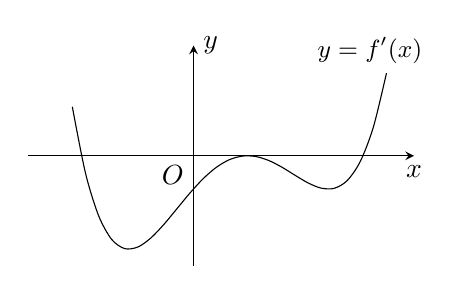
\begin{tikzpicture}[scale=0.7, >=stealth]
			\draw[->] (-3,0) -- (4,0) node[below] {$x$};
			\draw[->] (0,-2) -- (0,2) node[right] {$y$};
			\draw[domain=-2.2:3.5, smooth, variable=\x, black] plot ({\x}, {(\x-0.5)*(\x-1.5)*(\x-3)*(\x+2)*0.1-0.15});
			\node at (0,0) [below left] {$O$};
			\node at (3.2,1.5)[above]{\small $y=f'(x)$};
		\end{tikzpicture}
	\end{center}
	Số điểm cực tiểu của hàm số $y = f(x)$ là
	\choice
	{$3$}
	{$0$}
	{$2$}
	{\True $1$}
	\loigiai{		
		\begin{center}
			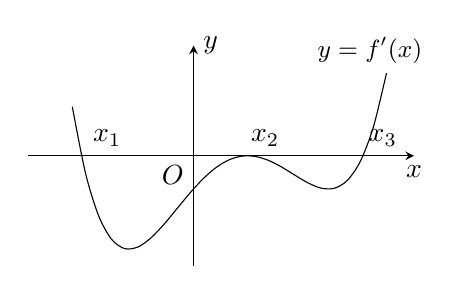
\begin{tikzpicture}[scale=0.7, >=stealth]
				\draw[->] (-3,0) -- (4,0) node[below] {$x$};
				\draw[->] (0,-2) -- (0,2) node[right] {$y$};
				\draw[domain=-2.2:3.5, smooth, variable=\x, black] plot ({\x}, {(\x-0.5)*(\x-1.5)*(\x-3)*(\x+2)*0.1-0.15});
				\node at (0,0) [below left] {$O$};
				\node at (3.2,1.5)[above]{\small $y=f'(x)$};
				\node[above right] at (-2,0) {$x_1$};
				\node[above] at (1.3,0) {$x_2$};
				\node[above right] at (3,0) {$x_3$};
			\end{tikzpicture}
		\end{center}
	Gọi $x_1, x_2, x_3$ lần lượt là hoành độ giao điểm của $y=f'(x)$ và trục hoành. Dựa vào đồ thị $f'(x)$, ta thấy $f'(x)$ đổi dấu từ dương sang âm tại $x_1$, không đổi dấu tại $x_2$ và từ âm sang dương tại $x_3$. Vậy, hàm số có $1$ điểm cực tiểu.
	}
\end{ex}

\begin{ex}%[Chuyên Lê Hồng Phong, Ninh Bình, Lần 3] %[Phan Chiến Thắng, 26-2-DuAnDeTHPT-2025-2026]%[2H2H1-2]
	Cho hình hộp $ABCD.A'B'C'D'$. Đặt $\vec{a} = \vec{AB}$, $\vec{b} = \vec{AD}$, $\vec{c} = \vec{AA'}$. Khẳng định nào sau đây đúng?
	\choice
	{$\vec{B'D} = \vec{a} - \vec{b} - \vec{c}$}
	{$\vec{B'D} = \vec{a} - \vec{b} + \vec{c}$}
	{$\vec{B'D} = \vec{a} + \vec{b} + \vec{c}$}
	{\True $\vec{B'D} = -\vec{a} + \vec{b} - \vec{c}$}
	\loigiai{
		Ta có $\vec{B'D} = \vec{B'B} + \vec{BD} = -\vec{AA'} + (\vec{AD} - \vec{AB}) = -\vec{c} + \vec{b} - \vec{a}$. }
\end{ex}

\begin{ex}%[Chuyên Lê Hồng Phong, Ninh Bình, Lần 3] %[Phan Chiến Thắng, 26-2-DuAnDeTHPT-2025-2026]%[2D4H1-4]
	Cho hàm số $F(x)$ thỏa mãn $\displaystyle\int x e^{2x} dx = F(x) + C$. Giá trị của biểu thức $P = F''(1) - 2F'(1)$ bằng
	\choice
	{$0$}
	{\True $e^2$}
	{$2e^2$}
	{$3e^2$}
	\loigiai{
		Ta có $F'(x) = x e^{2x}$. Suy ra $F''(x) = (x e^{2x})' = e^{2x} + 2x e^{2x}$.\\
		Vậy $P = F''(1) - 2F'(1) = (e^2 + 2e^2) - 2(e^2) = 3e^2 - 2e^2 = e^2$.
	}
\end{ex}

\begin{ex}%[Chuyên Lê Hồng Phong, Ninh Bình, Lần 3] %[Phan Chiến Thắng, 26-2-DuAnDeTHPT-2025-2026]%[1H8H6-2]
	Cho hình chóp tam giác đều $S.ABC$. Gọi $M$ là trung điểm của cạnh $BC$ như hình vẽ dưới đây. 
	\begin{center}
		\begin{tikzpicture}[scale=1, font=\footnotesize, line join=round, line cap=round, >=stealth]
			\def\ac{4} 
			\def\ab{2} 
			\def\h{4} 
			\def\gocA{50} 
			\coordinate[label=left:$A$] (A) at (0,0);
			\coordinate[label=right:$C$] (C) at (\ac,0);
			\coordinate[label=below left:$B$] (B) at (-\gocA:\ab);
			\coordinate[label=below right:$M$] (M) at ($(B)!.5!(C)$);
			\coordinate[label] (G) at ($(A)!2/3!(M)$);
			\coordinate[label=above:$S$] (S) at ($(G)+(90:\h)$);
			\draw (A)--(B)--(C)--(S)--cycle (S)--(B);
			\draw[dashed] (A)--(C);
			\foreach \diem in {A,B,C,S,M}	\fill (\diem)circle(1.5pt);
		\end{tikzpicture}
		
	\end{center}
	Góc phẳng nhị diện của góc nhị diện $[S, BC, A]$ là góc nào dưới đây?
	\choice
	{$\widehat{SAB}$}
	{$\widehat{SBM}$}
	{\True $\widehat{SMA}$}
	{$\widehat{SCA}$}
	\loigiai{
		Góc nhị diện $[S, BC, A]$ có hai mặt là $(SBC)$ và $(ABC)$.
		Vì $S.ABC$ là hình chóp đều nên $SA \perp BC$ và $MA \perp BC$.
		Góc giữa hai mặt phẳng là góc giữa hai đường thẳng $SM$ và $AM$ cùng vuông góc với giao tuyến $BC$ tại $M$.
		Vậy góc đó là $\widehat{SMA}$.
	}
\end{ex}

\begin{ex}%[Chuyên Lê Hồng Phong, Ninh Bình, Lần 3] %[Phan Chiến Thắng, 26-2-DuAnDeTHPT-2025-2026]%[1D2H3-3]
	Cho cấp số nhân $(u_n)$ có số hạng đầu $u_1 = 3$ và công bội $q = -2$. Số hạng thứ $5$ của cấp số nhân đã cho bằng
	\choice
	{$-5$}
	{$-48$}
	{\True $48$}
	{$-96$}
	\loigiai{
		Số hạng tổng quát của cấp số nhân là $u_n = u_1 \cdot q^{n-1}$.\\
		Số hạng thứ $5$ là $u_5 = u_1 \cdot q^4 = 3 \cdot (-2)^4 = 3 \cdot 16 = 48$.
	}
\end{ex}

\begin{ex}%[Chuyên Lê Hồng Phong, Ninh Bình, Lần 3] %[Phan Chiến Thắng, 26-2-DuAnDeTHPT-2025-2026]%[2D1H5-1]
	Đường cong trong hình vẽ dưới đây là đồ thị của một trong bốn hàm số được liệt kê ở bốn phương án A, B, C, D.
	\begin{center}
		\begin{tikzpicture}[scale=0.8, >=stealth]
			\draw[->] (-3,0) -- (4,0) node[below] {$x$};
			\draw[->] (0,-2) -- (0,4) node[right] {$y$};
			\draw (0,0) node[below right] {$O$};
			\draw (1,0) node[below right] {$1$};
			\draw (2,0) node[below] {$2$};
			\draw (0,3) node[left] {$3$};
			\draw (0,-1) node[left] {\small $-1$};
			\draw[dashed] (1,-2) -- (1,4) (2,0)--(2,3)--(0,3);
			\draw[dashed] (-2,-2) -- (3.5,3.5);
			\draw[domain=-1.7:0.6, smooth, variable=\x, blue, thick] plot ({\x}, {(\x*\x-\x+1)/(\x-1)});
			\draw[domain=1.4:3, smooth, variable=\x, blue, thick] plot ({\x}, {(\x*\x-\x+1)/(\x-1)});
		\end{tikzpicture}
	\end{center}
	Hỏi hàm số đó là hàm số nào dưới đây?
	\choice
	{\True $y = \dfrac{x^2 - x + 1}{x - 1}$}
	{$y = \dfrac{-x^2 + x - 1}{x - 1}$}
	{$y = \dfrac{x^2 - x - 1}{x - 1}$}
	{$y = \dfrac{x^2 + x + 1}{x + 1}$}
	\loigiai{
		Đồ thị hàm số có tiệm cận đứng là $x=1$, tiệm cận xiên là đường thẳng đi qua $(0,0)$. Đồ thị hàm số đi qua điểm $A(0;-1)$ và $B(2;3)$ nên hàm số thỏa mãn là $y = \dfrac{x^2 - x + 1}{x - 1}$.
	}
\end{ex}

\begin{ex}%[Chuyên Lê Hồng Phong, Ninh Bình, Lần 3] %[Phan Chiến Thắng, 26-2-DuAnDeTHPT-2025-2026]%[2H5H2-3]
	Trong không gian $Oxyz$, đường thẳng đi qua điểm $M(1; -2; 3)$ và vuông góc với mặt phẳng $(P): 2x - y + 3z - 5 = 0$ có phương trình chính tắc là
	\choice
	{$\dfrac{x - 1}{2} = \dfrac{y + 2}{1} = \dfrac{z - 3}{3}$}
	{$\dfrac{x + 1}{2} = \dfrac{y - 2}{-1} = \dfrac{z + 3}{3}$}
	{\True $\dfrac{x - 1}{2} = \dfrac{y + 2}{-1} = \dfrac{z - 3}{3}$}
	{$\dfrac{x - 2}{1} = \dfrac{y + 1}{-2} = \dfrac{z - 3}{3}$}
	\loigiai{
		Đường thẳng vuông góc với mặt phẳng $(P)$ nên nhận vectơ pháp tuyến của $(P)$ là $\vec{n} = (2; -1; 3)$ làm vectơ chỉ phương.
		Phương trình đường thẳng đi qua $M(1; -2; 3)$ có VTCP $\vec{u} = (2; -1; 3)$ là $\dfrac{x - 1}{2} = \dfrac{y + 2}{-1} = \dfrac{z - 3}{3}$.
	}
\end{ex}

\begin{ex}%[Chuyên Lê Hồng Phong, Ninh Bình, Lần 3] %[Phan Chiến Thắng, 26-2-DuAnDeTHPT-2025-2026]%[2D4H3-1]
	Gọi $S_1$ và $S_2$ là diện tích của hai hình phẳng giới hạn bởi đồ thị của hàm số $y = f(x)$ và trục hoành như hình vẽ dưới đây.
	\begin{center}
		\begin{tikzpicture}[scale=1,>=stealth]
			\draw[->] (-2,0) -- (5,0) node[right] {$x$};
			\draw[->] (0,-2.5) -- (0,2) node[above] {$y$};
			\draw[domain=-1.1:4.1, smooth, variable=\x] plot({\x}, {(\x-1)*(\x+1)*(\x-4)/4});
			\fill[pattern=north east lines, pattern color=black, opacity=0.4]
			plot[domain=-1:1, smooth] (\x, {(\x-1)*(\x+1)*(\x-4)/4})
			-- (1,0) -- (-1,0)-- cycle;
			\fill[pattern=crosshatch, pattern color=black, opacity=0.4]
			plot[domain=1:4, smooth] (\x, {(\x-1)*(\x+1)*(\x-4)/4})	-- (4,0) -- (1,0) -- cycle;
			\node[above left] at (-1,0){$-1$};
			\node[below right] at (4,0){$4$};
			\node[below left] (0,0) {$O$};
			\node at (-0.2,0.5) {$S_1$};
			\node at (2.5,-1) {$S_2$};
			\node at (4.3,0.5) {$y = f(x)$};
		\end{tikzpicture}
	\end{center}
	Tích phân $\displaystyle\int\limits_{-1}^{4} f(x)\mathrm{d}x$ bằng
	\choice
	{\True $S_1 - S_2$}
	{$S_1 + S_2$}
	{$-S_1 - S_2$}
	{$-S_1 + S_2$}
	\loigiai{	\begin{center}
			\begin{tikzpicture}[scale=1,>=stealth]
				\draw[->] (-2,0) -- (5,0) node[right] {$x$};
				\draw[->] (0,-2.5) -- (0,2) node[above] {$y$};
				\draw[domain=-1.1:4.1, smooth, variable=\x] plot({\x}, {(\x-1)*(\x+1)*(\x-4)/4});
				\fill[pattern=north east lines, pattern color=black, opacity=0.4]
				plot[domain=-1:1, smooth] (\x, {(\x-1)*(\x+1)*(\x-4)/4})
				-- (1,0) -- (-1,0)-- cycle;
				\fill[pattern=crosshatch, pattern color=black, opacity=0.4]
				plot[domain=1:4, smooth] (\x, {(\x-1)*(\x+1)*(\x-4)/4})	-- (4,0) -- (1,0) -- cycle;
				\node[above left] at (-1,0){$-1$} ;
				\node[below right] at (4,0){$4$};
				\node[below left] (0,0) {$O$};
				\node at (-0.2,0.5) {$S_1$};
				\node at (2.5,-1) {$S_2$};
				\node at (4.3,0.5) {$y = f(x)$};
				\node[below left] at (1,0) {$x_0$};
			\end{tikzpicture}
		\end{center}
	Ta có $\displaystyle\int\limits_{-1}^{4} f(x)\mathrm{d}x = \displaystyle\int\limits_{-1}^{x_0} f(x)\mathrm{d}x + \displaystyle\int\limits_{x_0}^{4} f(x)\mathrm{d}x$.\\
		Vì $f(x) \ge 0$ trên $[-1, x_0]$ nên $\displaystyle\int\limits_{-1}^{x_0} f(x)\mathrm{d}x = S_1$.\\
		Vì $f(x) \le 0$ trên $[x_0, 4]$ nên $\displaystyle\int\limits_{x_0}^{4} f(x)\mathrm{d}x = -S_2$.\\
		Vậy $\displaystyle\int\limits_{-1}^{4} f(x)\mathrm{d}x$ bằng $S_1 - S_2$.
	}
\end{ex}

\begin{ex}%[Chuyên Lê Hồng Phong, Ninh Bình, Lần 3] %[Phan Chiến Thắng, 26-2-DuAnDeTHPT-2025-2026]%[1D1H4-2]
	Tập xác định của hàm số $y = \dfrac{1}{\sin x} + \tan x$ là
	\choice
	{\True $\mathcal{D} = \mathbb{R} \setminus \left\{\dfrac{k\pi}{2} \mid k \in \mathbb{Z}\right\}$}
	{$\mathcal{D} = \mathbb{R} \setminus \left\{k2\pi \mid k \in \mathbb{Z}\right\}$}
	{$\mathcal{D} = \mathbb{R} \setminus \left\{k\pi \mid k \in \mathbb{Z}\right\}$}
	{$\mathcal{D} = \mathbb{R} \setminus \left\{\dfrac{\pi}{2} + k\pi \mid k \in \mathbb{Z}\right\}$}
	\loigiai{
		Điều kiện xác định $\heva{&\sin x \neq 0\\&\cos x \neq 0}\Leftrightarrow\heva{&x \neq k\pi\\&x \neq \dfrac{\pi}{2} + k\pi}\Leftrightarrow x\neq\dfrac{k\pi}{2}$, $k\in\mathbb{Z}$.
	}
\end{ex}
\Closesolutionfile{ans}

\cauds
\Opensolutionfile{ans}[ans/ans-26-2-NinhBinh-ChuyenLeHongPhong-L3-DS]
\begin{ex}%[Chuyên Lê Hồng Phong, Ninh Bình, Lần 3] %[Phan Chiến Thắng, 26-2-DuAnDeTHPT-2025-2026]%[2D6V2-4]
	Một dịch vụ truyền hình trực tuyến tại Việt Nam cung cấp $3$ gói đăng kí dịch vụ bao gồm gói \lq\lq Cơ bản\rq\rq, gói \lq\lq Tiêu chuẩn\rq\rq và gói \lq\lq Cao cấp\rq\rq. Những người sử dụng dịch vụ thông qua việc đóng phí hằng tháng được gọi là thuê bao. Mỗi thuê bao chỉ được chọn một trong ba gói dịch vụ trên. Theo thống kê của hệ thống: có $70\%$ số thuê bao là người từ $40$ tuổi trở xuống. Trong số những thuê bao từ $40$ tuổi trở xuống, có $20\%$ người chọn gói Cơ bản, $30\%$ người chọn gói Tiêu chuẩn và $50\%$ người chọn gói Cao cấp. Trong số những thuê bao trên $40$ tuổi, có $40\%$ người chọn gói Cơ bản, $40\%$ người chọn gói Tiêu chuẩn và $20\%$ người chọn gói Cao cấp.
	\choiceTF[1]
	{Nếu chọn ngẫu nhiên một thuê bao và biết người đó đăng kí gói Cao cấp, xác suất để thuê bao đó trên $40$ tuổi lớn hơn $15\%$}
	{Cần chọn ngẫu nhiên ít nhất $12$ thuê bao để xác suất có ít nhất một người trên $40$ tuổi lớn hơn $99\%$}
	{\True Xác suất để chọn ngẫu nhiên một thuê bao là người từ $40$ tuổi trở xuống và có đăng kí gói Cao cấp bằng $0{,}35$}
	{\True Xác suất để chọn ngẫu nhiên một thuê bao là người trên $40$ tuổi bằng $0{,}3$}
	\loigiai{Gọi $A$ là biến cố \lq\lq Thuê bao từ $40$ tuổi trở xuống\rq\rq, $B$ là biến cố \lq\lq Thuê bao trên $40$ tuổi\rq\rq. \\ Ta có $P(A) = 0{,}7$, $P(B) = 0{,}3$.
		\begin{itemchoice}
		\itemch Gọi $C$ là biến cố \lq\lq Thuê bao chọn gói Cao cấp\rq\rq. Ta có $P(C|A) = 0{,}5$, $P(C|B) = 0{,}2$. Ta cần tính $P(B\mid C)$.\\
		Ta có $P(C) = P(A)P(C|A) + P(B)P(C|B) = 0{,}7 \cdot 0{,}5 + 0{,}3 \cdot 0{,}2 = 0{,}35 + 0{,}06 = 0{,}41$.\\
		Vậy $P(B|C) = \dfrac{P(B)P(C|B)}{P(C)} = \dfrac{0{,}06}{0{,}41} \approx 0{,}1463 = 14{,}63\%$. Vậy phát biểu a) là Sai.
		\itemch Gọi $n$ là số thuê bao cần chọn. $D$ là biến cố trong $n$ thuê bao được chọn có ít nhất một thuê bao trên $40$ tuổi. Ta có \[P(D)=1-P(\overline{D})=1-(0,7)^n> 0,99\Leftrightarrow (0,7)^n<0,01\Leftrightarrow n>\log_{0,7}0,01\approx 12,9.\]
		Vậy cần chọn ít nhất $13$ thuê bao.
		\itemch Ta có $P(AC)=P(A)\cdot P(C\mid A)=0,7\cdot 0,5=0,35$.
		\itemch Ta có $P(B)=0,3$.
		\end{itemchoice}
	}
\end{ex}
\begin{ex}%[Chuyên Lê Hồng Phong, Ninh Bình, Lần 3] %[Phan Chiến Thắng, 26-2-DuAnDeTHPT-2025-2026]%[2H2C2-2]
	Đang có một buổi triển lãm hàng không tại sân bay thể thao. Xét trong hệ trục tọa độ $Oxyz$ (với mặt phẳng $(Oxy)$ là mặt đất, đơn vị đo chiều dài là mét), một khinh khí cầu được thả ra tại điểm $B(280; 600; 0)$. Khinh khí cầu bay lên theo phương thẳng đứng (cùng hướng với trục $Oz$) với vận tốc $5\text{ m/s}$, trời không có gió. Cùng lúc đó, một chiếc máy bay đang ở điểm $F(0; -1350; 650)$ bay với vận tốc $40\text{ m/s}$ dọc theo một đường thẳng song song với trục $Oy$, theo chiều dương của trục $Oy$. Khoảng cách an toàn tối thiểu giữa khinh khí cầu và máy bay phải luôn là $500\text{ m}$. Gọi $t$ (giây) là thời gian kể từ lúc khinh khí cầu bắt đầu được thả lên.
	\choiceTF[1]
	{\True Khoảng cách ngắn nhất giữa hai phương tiện bay xấp xỉ $490{,}81\text{ m}$}
	{Thời điểm đầu tiên khoảng cách an toàn bị vi phạm (nhỏ hơn mức quy định $500\text{ m}$) là đúng tại giây thứ $50$}
	{Tại thời điểm $t = 20$ giây, khoảng cách giữa hai phương tiện bay là $1300\text{ m}$}
	{\True Tại thời điểm $t$ (giây), tọa độ của chiếc máy bay là $F_t(0; -1350 + 40t; 650)$}
	\loigiai{
		\begin{itemchoice}
			\itemch Tọa độ khinh khí cầu và máy bay  tại thời điểm $t$ lần lượt là \[B_t(280; 600; 5t),F_t(0; -1350 + 40t; 650).\]
			Khoảng cách giữa máy bay và khinh khí cầu là \[B_tF_t =\sqrt{(280-0)^2 + (600 - (-1350 + 40t))^2 + (5t - 650)^2} =\sqrt{1625t^2 - 162500t + 4303400}.\]
			Khoảng cách ngắn nhất tại $t = \dfrac{162500}{2 \cdot 1625} = 50$ là $\sqrt{1625\cdot 50^2 - 162500\cdot 50 + 4303400} = \sqrt{240900} \approx 490{,}81$ m.
			\itemch Để khoảng cách an toàn bay bị vi phạm thì \[B_tF_t\leq 500\Leftrightarrow\sqrt{1625t^2 - 162500t + 4303400}\leq 500\Leftrightarrow 47{,}6\leq t\leq 52{,}3.\] 
			\itemch Tại $t=20$, thì $B_tF_t=\sqrt{1625\cdot 20^2 - 162500\cdot 20 + 4303400}\approx 1305$ m.
			\itemch Máy bay xuất phát tại $F(0; -1350; 650)$ với vận tốc $40$ m/s theo chiều dương trục $Oy$, nên tọa độ là $(0; -1350 + 40t; 650)$.
		\end{itemchoice}
	}
\end{ex}

\begin{ex}%[Chuyên Lê Hồng Phong, Ninh Bình, Lần 3] %[Phan Chiến Thắng, 26-2-DuAnDeTHPT-2025-2026]%[2D1V3-1]
	Cho hàm số $y = e^x(\sin x - \cos x)$.
	\choiceTF[1]
	{\True Giá trị lớn nhất của hàm số trên đoạn $[0; \pi]$ bằng $e^\pi$}
	{\True Đạo hàm của hàm số đã cho là $y' = 2e^x \sin x$}
	{\True Hàm số đạt cực tiểu tại điểm $x = 0$}
	{Các nghiệm của phương trình $y' = 0$ là $x = \dfrac{\pi}{2} + k\pi$ với $k \in \mathbb{Z}$}
	\loigiai{Ta có $y' = e^x(\sin x - \cos x) + e^x(\cos x + \sin x) = 2e^x \sin x$.\\
		Do đó $y'=0\Leftrightarrow \sin x=0\Leftrightarrow x=k\pi,k\in\mathbb{Z}$.
		\begin{itemchoice}
			\itemch Trên đoạn $[0,\pi]$ ta có $y(0) = -1$, $y(\pi) = e^\pi(0 - (-1)) = e^\pi$. Vậy, giá trị lớn nhất là $e^\pi$.
			\itemch Ta có $y' = e^x(\sin x - \cos x) + e^x(\cos x + \sin x) = 2e^x \sin x$.
			\itemch Ta có $y''=2e^x(\sin x+\cos x)$ nên $y''(0) = 2>0$. Vậy $x=0$ là điểm cực tiểu của hàm số.
			\itemch Các nghiệm của phương trình $y' = 0$ là $x=k\pi, k\in\mathbb{Z}$.
		\end{itemchoice}
	}
\end{ex}

\begin{ex}%[Chuyên Lê Hồng Phong, Ninh Bình, Lần 3] %[Phan Chiến Thắng, 26-2-DuAnDeTHPT-2025-2026]%[1D6V4-6]
	Trung bình mỗi người trưởng thành ở Việt Nam tiêu thụ khoảng $200$ mg caffeine mỗi ngày. Sau khi uống, caffeine đi vào máu và được cơ thể phân giải theo thời gian. Diễn biến lượng caffeine trong máu sau khi uống được mô tả bởi hàm số mũ có dạng $f(t) = A \cdot \mathrm{e}^{k \cdot t}$, trong đó $A$ là lượng caffeine ban đầu (tính bằng mg), $t$ là thời gian kể từ lúc uống (tính bằng giờ), và $k$ là hằng số phân giải. Một người uống một tách cà phê chứa $120$ mg caffeine. Biết rằng cứ sau khoảng $3$ giờ thì lượng caffeine trong cơ thể người này lại giảm đi một nửa.
	\choiceTF[1]
	{\True Hàm số mô tả lượng caffeine trong máu của người đó sau $t$ giờ có phương trình $f(t) = 120 \cdot e^{-\tfrac{\ln 2}{3} \cdot t}$}
	{Sau $6$ giờ kể từ lúc uống, lượng caffeine còn lại trong máu người đó là $40$ mg}
	{\True Kể từ lúc uống, thời gian để lượng caffeine trong máu phân giải hết $\dfrac{7}{8}$ lượng ban đầu là $9$ giờ}
	{Một thanh niên uống một lon nước tăng lực chứa $160$ mg caffeine có cùng chu kì bán rã như trên. Biết rằng để không bị mất ngủ, lượng caffeine trong cơ thể không được vượt quá $20\text{ mg}$. Nếu thanh niên này dự định đi ngủ lúc $22$ giờ thì thời điểm muộn nhất có thể uống lon nước tăng lực đó là lúc $14$ giờ cùng ngày}
	\loigiai{Theo bài ra ta có $f(3)=\dfrac{A}{2}\Leftrightarrow \dfrac{A}{2}=A\cdot\mathrm{e}^{3k}\Leftrightarrow k=-\dfrac{\ln 2}{3}$.
		\begin{itemchoice}
			\itemch $f(t) = 120 \cdot \mathrm{e}^{-\frac{\ln 2}{3}t}$.
			\itemch $f(6) = 120 \cdot \mathrm{e}^{-2\ln 2} = 120 \cdot\dfrac{1}{4} = 30$ mg. 
			\itemch Phân giải hết $\dfrac{7}{8}$ nghĩa là còn lại $\dfrac{1}{8}$ lượng caffeine ban đầu. Ta có \[120 \cdot 2^{-\tfrac{t}{3}} = \dfrac{120}{8} \Rightarrow \dfrac{t}{3} = 3 \Rightarrow t = 9.\] 
			\itemch Ta có $160 \cdot 2^{-\tfrac{t}{3}} \le 20 \Leftrightarrow 2^{-\tfrac{t}{3}} \le \dfrac18 \Leftrightarrow \dfrac t3 \ge 3 \Leftrightarrow t \ge 9$ giờ. Từ $22$ giờ lùi lại $9$ giờ là $13$ giờ. 
		\end{itemchoice}
	}
\end{ex}
\Closesolutionfile{ans}

\Opensolutionfile{ans}[ans/ans-26-2-NinhBinh-ChuyenLeHongPhong-L3-KQ]
\caukq

\begin{ex}%[Chuyên Lê Hồng Phong, Ninh Bình, Lần 3] %[Phan Chiến Thắng, 26-2-DuAnDeTHPT-2025-2026]%[2D4C3-1]
	Một logo được thiết kế trên hệ trục tọa độ $Oxy$ (với đơn vị trên các trục là mét) gồm các đường $(C_1): y = x^2$, $(C_2): y = 2x$ và $(C_3): y = f(x)$. Lấy điểm $P(a; a^2)$ thuộc $(C_1)$ với $a \in [0; 1]$. Đường thẳng qua $P$ song song với trục hoành cắt $(C_2)$ tại $Q$ và đường thẳng qua $P$ song song với trục tung cắt $(C_3)$ tại $R$. Gọi $S_1$ là diện tích hình phẳng giới hạn bởi $(C_1), (C_2), PQ$ và $S_2$ là diện tích hình phẳng giới hạn bởi $(C_1), (C_3), PR$. Biết yêu cầu thiết kế là $S_1 = S_2$ với mọi $a \in [0; 1]$. Phần hình phẳng giới hạn bởi $(C_3)$ và trục hoành được lắp kính phát sáng. 
	\begin{center}
		\begin{tikzpicture}[scale=4,>=stealth]
			\draw[->] (-0.05,0) -- (1.15,0) node[above] {$x$};
			\draw[->] (0,-0.25) -- (0,1.15) node[right] {$y$};
			\draw (0,0) rectangle (1,1);
			\draw[blue, domain=0:1, samples=100] plot (\x,{\x*\x}) node[right] {$(C_1)$};
			\draw[red!70!black, domain=0:0.5, samples=100] plot (\x,{2*\x}) node[above] {$(C_2)$};
			\draw[cyan!60!black, domain=0:1, samples=100]plot (\x,{-0.35*\x*(1-\x)});
			\node[below] at (0.3,-0.1) {$(C_3)$};
			\coordinate (P) at (0.72,{0.72*0.72});
			\fill (P) circle (0.2pt) node[right]{$P$};
			\coordinate (Q) at ({0.72*0.72/2},{0.72*0.72});
			\fill (Q) circle (0.2pt) node[left] {$Q$};
			\coordinate (R) at (0.72,{-0.35*0.72*(1-0.72)});
			\fill (R) circle (0.2pt) node[below] {$R$};
			\draw[dashed] (Q) -- (P);
			\draw[dashed] (P) -- (R);
			%tô miền giới hạn
			\fill[green!10]	(0,0)-- plot[domain=0:0.72,samples=100] (\x,2*\x)--(Q)--plot[domain=0.72:0,samples=100] (\x,\x*\x)--(P)-- cycle;
			\fill[pattern=north east lines]	(0,0)-- plot[domain=0:0.72,samples=100] (\x,\x*\x)--(P)--plot[domain=0.72:0,samples=100] (\x,{-0.35*\x*(1-\x)})--(R)-- cycle;
			\fill[pattern=crosshatch](0,0)--plot[domain=0:0.72,samples=100] (\x,{-0.35*\x*(1-\x)})--(1,0);
			% Nhãn miền
			\node at (0.3,0.3) {$S_1$};
			\node at (0.5,0.1) {$S_2$};
			\node[left] at (0,1) {$1$};
			\node[below] at (1,0) {$1$};
			\node[below left] at (0,0) {$O$};
			% Chú thích kính phát sáng
			\draw[->] (0.93,-0.18) -- (0.78,-0.01);
			\node[below right] at (0.93,-0.18) {\small Kính phát sáng};
			
		\end{tikzpicture}
	\end{center}
	Biết chi phí loại kính này là $12$ triệu đồng/m$^2$. Tổng chi phí thi công phần kính phát sáng là bao nhiêu triệu đồng?
	\par\shortans{1}
	\loigiai{\begin{center}
			\begin{tikzpicture}[scale=4,>=stealth]
				\draw[->] (-0.05,0) -- (1.15,0) node[above] {$x$};
				\draw[->] (0,-0.25) -- (0,1.15) node[right] {$y$};
				\draw (0,0) rectangle (1,1);
				%==== C1
				\draw[blue, domain=0:1, samples=100] plot (\x,{\x*\x}) node[right] {$(C_1)$};
				%===== C2
				\draw[red!70!black, domain=0:0.5, samples=100] plot (\x,{2*\x}) node[above] {$(C_2)$};
				%===== C3
				\draw[cyan!60!black, domain=0:1, samples=100]plot (\x,{-0.35*\x*(1-\x)});
				\node[below] at (0.3,-0.1) {$(C_3)$};
				%Điểm
				\coordinate (P) at (0.72,{0.72*0.72});
				\fill (P) circle (0.2pt) node[right]{$P$};
				%==
				\coordinate (yP) at (0,{0.72*0.72});
				\fill (yP) circle (0.2pt) node[left]{$a^2$};
				%==				
				\coordinate (Q) at ({0.72*0.72/2},{0.72*0.72});
				\fill (Q) circle (0.2pt) node[above left] {$Q$};
				%==
				\coordinate (R) at (0.72,{-0.35*0.72*(1-0.72)});
				\fill (R) circle (0.2pt) node[below] {$R$};
				%==
				\draw[dashed] (yP)--(Q) -- (P);
				\draw[dashed] (P) -- (R);
				%tô miền giới hạn
				
				\fill[green!10]	(0,0)-- plot[domain=0:0.72,samples=100] (\x,2*\x)--(Q)--plot[domain=0.72:0,samples=100] (\x,\x*\x)--(P)-- cycle;
				%==
				\fill[pattern=north east lines]	(0,0)-- plot[domain=0:0.72,samples=100] (\x,\x*\x)--(P)--plot[domain=0.72:0,samples=100] (\x,{-0.35*\x*(1-\x)})--(R)-- cycle;
				%==
				\fill[pattern=crosshatch](0,0)--plot[domain=0:0.72,samples=100] (\x,{-0.35*\x*(1-\x)})--(1,0);
				% Nhãn miền
				\node at (0.3,0.3) {$S_1$};
				\node at (0.5,0.1) {$S_2$};
				\node[left] at (0,1) {$1$};
				\node[below] at (1,0) {$1$};
				\node[below left] at (0,0) {$O$};
				% Chú thích kính phát sáng
				\draw[->] (0.93,-0.18) -- (0.78,-0.01);
				\node[below right] at (0.93,-0.18) {\small Kính phát sáng};
				
			\end{tikzpicture}
			\end{center}
		Ta có $P(a; a^2)$. Gọi $d$ là đường thẳng qua $P$ song song với trục hoành có phương trình $y = a^2$.\\
		Theo bài ra, $d$ cắt $(C_2)\colon y = 2x$ tại $Q$ có hoành độ $x_Q = \dfrac{a^2}{2}$.\\ 
		+ Ta tính $S_1$ như sau.\\
		Từ $(C_1)$ ta có $x=\sqrt{y}$ và $(C_2)$ ta có $x=\dfrac{y}{2}$. Lúc này, $S_1 = \displaystyle\int\limits_{0}^{a^2} \left(\sqrt{y}-\dfrac{y}{2}\right)\mathrm{d}y =\dfrac{2}{3}a^3-\dfrac{a^4}{4}$.\\
		+ Tính $S_2$. Ta có $S_2 = \displaystyle\int\limits_{0}^{a} \left(x^2 - f(x)\right)\mathrm{d}x=\dfrac{a^3}{3}-\displaystyle\int\limits_{0}^{a} f(x)\mathrm{d}x$. \\
		Theo bài ra, ta có $S_1=S_2$ nên $\dfrac{a^3}{3}-\displaystyle\int\limits_{0}^{a} f(x)\mathrm{d}x= S_1 \Leftrightarrow \displaystyle\int\limits_{0}^{a} f(x)\mathrm{d}x = -\dfrac{a^3}{3} +\dfrac{a^4}{4}$.\\
		Đạo hàm hai vế theo $a$ cho ta $f(a) = a^3-a^2$.\\
		Diện tích phần kính là $S = \displaystyle\int\limits_{0}^{1} |f(x)| \mathrm{d}x = \displaystyle\int\limits_{0}^{1} |x^3 - x^2|\mathrm{d}x = \dfrac{1}{12}$ (m$^2$).\\
		Chi phí là $\dfrac{1}{12} \times 12 = 1$ triệu đồng.
	}
\end{ex}

\begin{ex}%[Chuyên Lê Hồng Phong, Ninh Bình, Lần 3] %[Phan Chiến Thắng, 26-2-DuAnDeTHPT-2025-2026]%[2H5V3-2]
	Một quả bóng hình cầu có bán kính $r$ đang được treo trong một góc của tường nhà. Một điểm $B$ cố định nằm trên mép hai bờ tường và cách mặt đất $56$ cm, sợi dây treo quả bóng có độ dài $AB = 20$ cm và đây cũng là độ dài ngắn nhất nối điểm $B$ với mặt xung quanh của quả bóng. 
	\begin{center}
		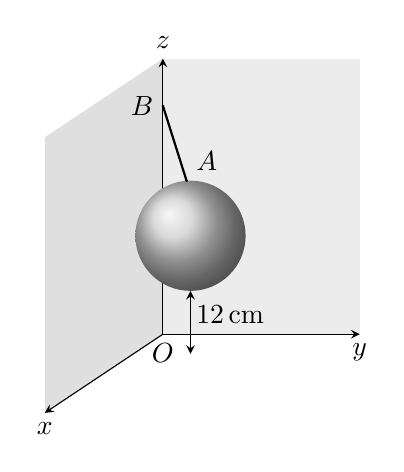
\begin{tikzpicture}[scale=0.5,>=stealth]
			% Hai mặt tường
			\fill[gray!15] (0,0) rectangle (5,7);
			\fill[gray!25] (-3,-2) -- (0,0) -- (0,7) -- (-3,5);
			
			% Trục tọa độ
			\draw[->] (0,0) -- (-3,-2) node[below] {$x$};
			\draw[->] (0,0) -- (5,0) node[below] {$y$};
			\draw[->] (0,0) -- (0,7) node[above] {$z$};
			
			% Quả bóng tiếp xúc hai tường
			\shade[ball color=gray!40] (0.7,2.5) circle (1.4);
			
			% Gốc tọa độ
			\node[below] at (0,0) {$O$};
			
			% Điểm B
			\coordinate (B) at (0,5.8);
			\fill (B) circle (1pt);
			\node[left] at (B) {$B$};
			
			% Điểm A trên mặt cầu
			\coordinate (A) at (0.6,3.9);
			\fill (A) circle (1pt);
			\node[above right] at (A) {$A$};
			
			% Dây treo
			\draw[thick] (B)--(A);
			
			% Kí hiệu 12cm
			\draw[<->] (0.7,-0.5) -- (0.7,1.1);
			\node[right] at (0.6,0.5) {$12\,\mathrm{cm}$};
		\end{tikzpicture}
	\end{center}
Biết rằng quả bóng tiếp xúc với hai bên bờ tường và điểm thấp nhất của quả bóng cách mặt đất $12$ cm. Hỏi quả bóng có đường kính là bao nhiêu cm?
	\par\shortans{$32$}
	\loigiai{
		Gọi $I$ là tâm quả bóng, $r$ là bán kính. Quả bóng tiếp xúc với hai tường và cách sàn $12$ cm nên tâm $I$ có tọa độ $(r, r, r+12)$.\\
		Khoảng cách từ $B(0,0,56)$ đến tâm $I$ là $BI = \sqrt{r^2 + r^2 + (56 - (r+12))^2} = \sqrt{2r^2 + (44-r)^2}$.\\
		Vì $AB = 20$ là khoảng cách ngắn nhất từ $B$ đến mặt cầu nên $BI = AB + r = 20 + r$.\\
		Từ đó ta có $\sqrt{2r^2 + (44-r)^2} = 20+r \Leftrightarrow r^2 - 64r + 768 = 0 \Leftrightarrow (r-16)(r-48) = 0$.\\
		Vì $r < 44$ nên $r = 16$. Vậy đường kính quả bóng hình cầu là $2r = 32$ cm.
	}
\end{ex}

\begin{ex}%[Chuyên Lê Hồng Phong, Ninh Bình, Lần 3] %[Phan Chiến Thắng, 26-2-DuAnDeTHPT-2025-2026]%[2D1V3-6]
	Chi phí đầu tư ban đầu để xây dựng một nhà máy sản xuất xe máy điện là $840$ tỷ đồng. Bộ phận nghiên cứu thị trường ước tính rằng: lượng cầu đối với dòng xe này phụ thuộc vào giá bán theo hàm số $x = 100 - 2p$; trong đó $p$ (triệu đồng) là giá niêm yết của mỗi chiếc và $x$ (nghìn chiếc) là số lượng xe bán ra trong một năm. Chi phí để sản xuất $x$ nghìn chiếc xe trong một năm (không bao gồm vốn đầu tư xây dựng nhà máy) được cho bởi hàm số $C(x) = 0,5x^2 + 10x + 50$ (tỷ đồng). Biết rằng nhà máy phải đóng thuế thu nhập doanh nghiệp là $20\%$ trên lợi nhuận hàng năm (doanh thu trừ đi chi phí sản xuất). Giả sử nhà máy luôn định giá $p$ sao cho lợi nhuận sau thuế đạt mức cao nhất. Hỏi với chiến lược giá tối ưu đó, nhà máy sẽ thu hồi được toàn bộ vốn đầu tư ban đầu sau bao nhiêu năm hoạt động?
	\par\shortans{3}
	\loigiai{Ta có $x = 100 - 2p$ suy ra $p = 50 - 0,5x$ (triệu đồng).\\
		Doanh thu $R(x) = p \cdot x = (50 - 0,5x)x = 50x - 0,5x^2$ (tỷ đồng).\\
		Lợi nhuận trước thuế $L(x) = R(x) - C(x) = 50x - 0,5x^2 - (0,5x^2 + 10x + 50) = -x^2 + 40x - 50$.\\
		Lợi nhuận sau thuế $L_s(x) = 0,8(-x^2 + 40x - 50) = -0,8x^2 + 32x - 40$.\\
		Hàm $L_s(x)$ là hàm số bậc hai hệ số $a<0$ nên đạt cực đại tại $x = \dfrac{-32}{2(-0,8)} = 20$.\\
		Lợi nhuận tối đa $L_s(20) = -0,8(400) + 32(20) - 40 = -320 + 640 - 40 = 280$ tỷ đồng/năm.\\
		Số năm thu hồi vốn $\dfrac{840}{240} = 3$ năm.
	}
\end{ex}

\begin{ex}%[Chuyên Lê Hồng Phong, Ninh Bình, Lần 3] %[Phan Chiến Thắng, 26-2-DuAnDeTHPT-2025-2026]%[1H8V7-2]
	Cho hình chóp $S.ABC$ có các mặt bên $SAB$ và $SAC$ là các tam giác đều cạnh bằng $3\sqrt{2}$, góc $\widehat{BAC} = 90^\circ$. Tính thể tích $V$ của khối chóp $S.ABC$.
	\par\shortans{$9$}
	\loigiai{
		\begin{center}
			\begin{tikzpicture}[scale=1, font=\footnotesize, line join=round, line cap=round, >=stealth]
				\def\ac{4} % cạnh AC
				\def\ab{3} % cạnh AB
				\def\h{5} % chiều cao
				\def\gocA{30} % góc A của đáy
				\coordinate[label=left:$B$] (B) at (0,0);
				\coordinate[label=right:$A$] (A) at (\ac,0);
				\coordinate[label=below left:$C$] (C) at (-\gocA:\ab);
				\coordinate[label=below left:$M$] (M) at ($(C)!.5!(B)$); 
				\coordinate[label=above left:$S$] (S) at ($(M)+(90:\h)$);
				\draw (A)--(C)--(B)--(S)--cycle (M)--(S)--(C);
				\draw[dashed] (B)--(A)--(M);
				\foreach \diem in {A,B,C,S,M}	\fill (\diem)circle(1.5pt);
				\newcommand{\gocv}[4][black]{\draw[#1] ($(#3)!5pt!(#2)$)--($(#3)!2!($($(#3)!5pt!(#2)$)!.5!($(#3)!5pt!(#4)$)$)$)--($(#3)!5pt!(#4)$);}
				\gocv{S}{M}{A}
			\end{tikzpicture}
			
		\end{center}
	Theo bài ra ta có $SA = SB = SC = 3\sqrt{2}$. Gọi $M$ là trung điểm $BC$.\\
	Tam giác $ABC$ vuông cân tại $A$ có $AB = AC = 3\sqrt{2}$ nên $BC = \sqrt{(3\sqrt{2})^2 + (3\sqrt{2})^2} = 6$.\\
	Ngoài ra, $AM = \dfrac{1}{2}BC = 3$.\\
	Vì $SA=SB=SC$ nên hình chiếu của $S$ lên $(ABC)$ là tâm đường tròn ngoại tiếp $\triangle ABC$, chính là trung điểm $M$ của $BC$.\\
	Trong tam giác $SAM$ vuông tại $M$ ta có $SM^2 = SA^2 - AM^2 = (3\sqrt{2})^2 - 3^2 = 9$ suy ra $SM = 3$.\\
	Chiều cao $h = SM = 3$. Diện tích đáy $S_{ABC} = \dfrac{1}{2} \cdot 3\sqrt{2} \cdot 3\sqrt{2} = 9$.\\
	Thể tích $V = \dfrac{1}{3} \cdot 9 \cdot 3 = 9$.
	}
\end{ex}

\begin{ex}%[Chuyên Lê Hồng Phong, Ninh Bình, Lần 3] %[Phan Chiến Thắng, 26-2-DuAnDeTHPT-2025-2026]%[2D6C1-4]
	Có $3$ chiếc hộp trống được kí hiệu là $A$, $B$ và $C$. Người ta thực hiện một phép thử như sau: Gieo một con xúc xắc cân đối và đồng chất, gọi $k$ là số chấm xuất hiện. Mỗi lần gieo, người ta lấy đúng $2$ quả bóng để cho vào các hộp theo quy tắc: nếu $k \le 2$ thì cho cả $2$ quả bóng vào hộp $A$; nếu $3 \le k \le 5$ thì cho $1$ quả bóng vào hộp $A$ và $1$ quả bóng vào hộp $B$; nếu $k = 6$ thì cho $1$ quả bóng vào hộp $B$ và $1$ quả bóng vào hộp $C$. Thực hiện lặp lại phép thử trên $2$ lần. Biết rằng sau $2$ lần gieo, số bóng có trong hộp $A$ là một số chẵn. Tính xác suất để số bóng trong hộp $B$ nhiều hơn số bóng trong hộp $C$.
	\shortans{$0{,}5$}
	\loigiai{
		Gọi $x_i$ là số bóng vào hộp $A$ sau lần gieo $i$, $x_i \in \{2, 1, 0\}$.
		Tổng số bóng hộp $A$ là $S_A = x_1 + x_2$ và $S_A \in \{0, 2, 4\}$.\\
		Các trường hợp $S_A$ chẵn:\\
		- $S_A = 0$: $(x_1, x_2) = (0, 0) \Rightarrow k_1=6, k_2=6$. Xác suất $P_0 = \dfrac{1}{36}$.\\
		- $S_A = 2$: $(x_1,x_2)\in\left\{(2,0), (0,2), (1,1)\right\}$. Xác suất $P_1=\dfrac{2}{6}\cdot\dfrac{1}{6}+\dfrac{1}{6}\cdot\dfrac{2}{6}+ \dfrac{3}{6}\cdot\dfrac{3}{6}=\dfrac{13}{36}$.\\
		- $S_A = 4$: $(x_1,x_2)=(2,2)$. Xác suất $P_2=\dfrac{4}{36}$.\\
		Xác suất để $S_A$ chẵn là $P=\dfrac{1}{36}+\dfrac{13}{36}+\dfrac{4}{36}=\dfrac{18}{36} = \dfrac{1}{2}$.\\
		Xét số bóng hộp $B$ là $S_B$ và số bóng hộp $C$ là $S_C$.\\
		- $S_A=0 \Rightarrow (k_1, k_2)=(6,6) \Rightarrow S_B=2, S_C=2 \Rightarrow S_B = S_C$, trường hợp này không thỏa mãn.\\
		- $S_A=2$:\\
		+ $(x_1,x_2)=(2,0)\Rightarrow (k_1, k_2) \in \{(1,6), (2,6)\} \Rightarrow S_B=1, S_C=1$, trường hợp này không thỏa mãn.\\
		+ $(x_1,x_2)=(0,2)\Rightarrow (k_1, k_2) \in \{(6,1), (6,2)\} \Rightarrow S_B=1, S_C=1$, trường hợp này cũng không thỏa mãn.\\
		+ $(x_1,x_2)=(1,1)\Rightarrow (k_1, k_2) \in \{(3,3), (3,4), (3,5), (4,3), (4,4), (4,5), (5,3), (5,4), (5,5)\} \Rightarrow S_B=2, S_C=0 \Rightarrow S_B > S_C$, trường hợp này thỏa mãn.\\
		- $S_A=4: (x_1,x_2)=(2,2) \Rightarrow S_B=0, S_C=0$, trường hợp này không thỏa mãn.\\
		Gọi $A$ là biến cố số bóng trong hộp $A$ là chẵn, $B$ là biến cố số bóng trong hộp $B$ nhiều hơn số bóng trong hộp $C$. Ta cần tính $P(B\mid A)$.
		Ta có $P(B\mid A)=\dfrac{P(AB)}{P(A)}=\dfrac{\dfrac{9}{36}}{\dfrac{1}{2}}= \dfrac{1}{2}= 0{,}5$.
	}
\end{ex}

\begin{ex}%[Chuyên Lê Hồng Phong, Ninh Bình, Lần 3] %[Phan Chiến Thắng, 26-2-DuAnDeTHPT-2025-2026]%[1D7C1-4]
	Một chậu nước có lòng chậu là hình nón cụt, đáy nhỏ bán kính $2$ dm, miệng chậu bán kính $4$ dm, chiều cao lòng chậu $4$ dm. Trong chậu có sẵn một viên bi sắt đường kính $4$ dm đặt ở đáy. Người ta đổ nước vào chậu với lưu lượng không đổi $1{,}5$ dm$^3$/s. Hỏi tại thời điểm mực nước đạt độ cao bằng $\dfrac{3}{4}$ đường kính viên bi, tốc độ tăng chiều cao mực nước là bao nhiêu (dm/s)? (Làm tròn đến hàng phần trăm).
	\par\shortans{$0{,}05$}
	\loigiai{
		\begin{center}
				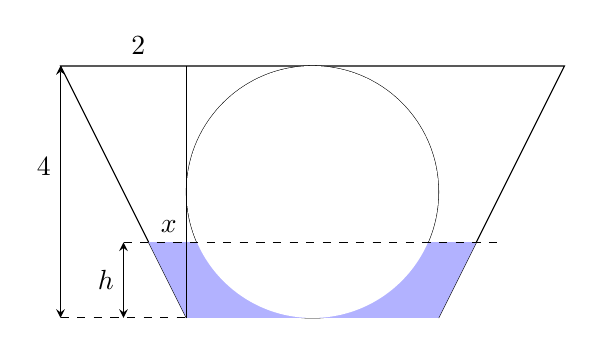
\begin{tikzpicture}[scale=0.8,>=stealth]
				
				%----------------------
				% Thông số
				%----------------------
				\def\H{4}      % chiều cao nón cụt
				\def\R{4}      % bán kính miệng
				\def\r{2}      % bán kính đáy nhỏ
				\def\rb{2}     % bán kính viên bi
				\def\h{1.2}    % mực nước, h < rb
				
				% Thành chậu (mặt cắt dọc)
				\draw[]
				(-\r,0)--(-\R,\H)--(\R,\H)--(\r,0);
				
				% Đáy chậu
				\draw[] (-\r,0)--(\r,0);
				
				% Viên bi
				\draw[] (0,\rb) circle (\rb);
				
				%----------------------
				% Miền nước
				%----------------------
				\begin{scope}
					
					% clip bên trong chậu
					\clip
					(-\r,0)--(-\R,\H)--(\R,\H)--(\r,0)--cycle;
					
					% tô phần nước dưới độ cao h
					\fill[blue!30]
					(-5,0) rectangle (5,\h);
					
					% bỏ phần bên trong viên bi
					\fill[white]
					(0,\rb) circle (\rb);
					
				\end{scope}
				
				% Đường mực nước
				\draw[dashed] (-3,\h)--(3,\h) (-4,0)--(-\r,0);
				\draw[<->] (-3,\h)--(-3,0);
				\draw[<->] (-\R,0)--(-\R,\H);
				% Ký hiệu h
				\node[left] at (-3,0.5*\h) {$h$};
				\node[left] at (-4,2*\h) {$4$};
				\node[left] at (-2.5,3.6*\h) {$2$};
				\draw (-\r,0)--(-\r,\R) (-\r,\h)node[above left ]{$x$};
				
			\end{tikzpicture}
		\end{center}
		Bán kính viên bi $R_b = 2$ dm. Hình nón cụt có bán kính đáy $r_1=2$ dm, $r_2=4$ dm và chiều cao $h_c=4$ dm. Thể tích nước $V_n = V_{c} - V_{b}$, trong đó $V_c$, $V_b$ lần lượt là thể tích chậu và của viên bi.\\ Xét tại thời điểm mực nước dâng cao lên $h$ dm.\\
		Ta có $\dfrac{x}{h}=\dfrac{2}{4}$ suy ra $x=\dfrac{h}{2}$ nên bán kính mặt nước tại đó là $r_n=2+0{,}5h$. \\
		Ta có $V_{c} = \dfrac{1}{3}\pi h \left(r_1^2 + r_1r_n + r_n^2\right) = \dfrac{1}{3}\pi h \left(4 + 2(2+0,5h) + (2+0,5h)^2\right)=\dfrac{1}{3}\pi h(12+3h+0{,}25h^2)$.\\
		Thể tích chỏm cầu $V_{b} = \dfrac{1}{3}\pi h^2 (3R_b - h) = \dfrac{1}{3}\pi h^2 (6 - h)$.\\
		Từ đó ta có thể tích phần nước là $$V_n = \dfrac{1}{3}\pi [h(12 + 3h + 0,25h^2) - (6h^2 - h^3)] = \dfrac{1}{3}\pi (12h - 3h^2 + 1,25h^3).$$
		Lấy đạo hàm hai vế theo thời gian $t$, ta có $V'_n(t) = \dfrac{1}{3}\pi (12h'(t) - 6h(t)\cdot h'(t) + 3,75h^2(t)\cdot h'(t))$.\\
		Tại $h=3$ ta có $\dfrac{1}{3}\pi (12h'(t) - 6h(t)\cdot h'(t) + 3,75h^2(t)\cdot h'(t)) = 1,5$.\\
		Do đó $\dfrac{1}{3}\pi (12h'(t)-18h'(t)+33{,}75h'(t)) = 1,5$ nên $9,25\pi\cdot h'(t) = 1,5\Rightarrow h'(t) = \dfrac{1,5}{9,25\pi} \approx 0,05$.
	}
\end{ex}

\Closesolutionfile{ans}
\newpage
\indapan{6}{ans/ans-26-2-NinhBinh-ChuyenLeHongPhong-L3-TN}
\indapan{4}{ans/ans-26-2-NinhBinh-ChuyenLeHongPhong-L3-DS}
\indapan{6}{ans/ans-26-2-NinhBinh-ChuyenLeHongPhong-L3-KQ}
